\documentclass{beamer}
\begin{document}
\begin{frame}
\title{Validation plots for ttH BSM high mass samples (s+t channel)}
\author{Hui-Chi Lin (UMich), Meng-Ju Tsai (UMich), Philipp Gadow (CERN)}
\date{\today}
\maketitle
\end{frame}
\begin{frame}
\frametitle{Introduction}
\begin{itemize}
\item Study of ttH signal samples on parton and particle/event level.
\begin{itemize}
\item Samples studied range from 1 TeV to 3 TeV with 100 GeV spacing in mass.
\item Both s-channel and t-channel simulations were conducted.
\item Utilized the release AthGeneration,21.6.106 for the generation of samples.
\end{itemize}
\item Link to the code used for producing results: \url{https://github.com/philippgadow/atlas-run3-multitops-bsm-joboptions/tree/r21}
\end{itemize}
\end{frame}
\begin{frame}
\frametitle{Signal Mass and Width}
\begin{table}
\begin{tabular}{cc}
\textbf{Signal Mass} & \textbf{Signal Width} \\
\textbf{(GeV)} & \textbf{(GeV)} \\
1000 & 30 \\
1100 & 40 \\
1200 & 40 \\
1300 & 50 \\
1400 & 50 \\
1500 & 60 \\
1750 & 90 \\
2000 & 100 \\
2250 & 110 \\
2500 & 125 \\
\end{tabular}
\end{table}
\end{frame}
\begin{frame}
\frametitle{Sample: ttH 1000 GeV - parton level plots}
\begin{columns}
\column{0.3\textwidth}
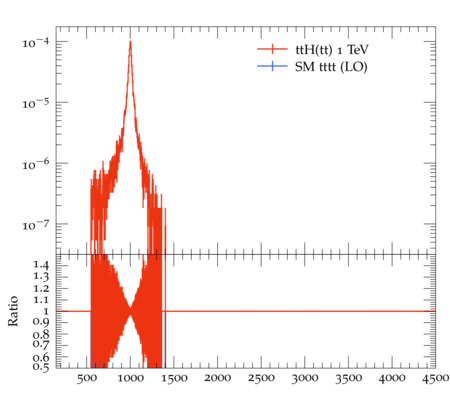
\includegraphics[width=\textwidth]{../plots/ttH_1000/tttt_ttH/Inclusive_mH.png}\\
\textit{\small Inclusive mH}
\column{0.3\textwidth}
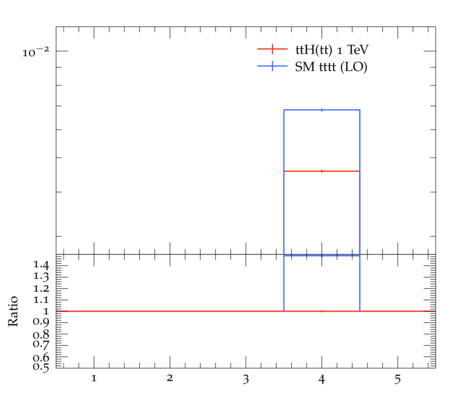
\includegraphics[width=\textwidth]{../plots/ttH_1000/tttt_ttH/Inclusive_nTop.png}\\
\textit{\small Inclusive nTop}
\column{0.3\textwidth}
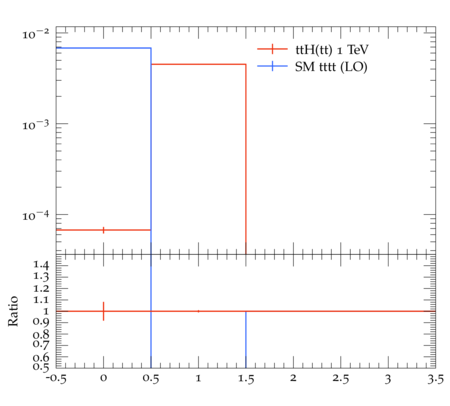
\includegraphics[width=\textwidth]{../plots/ttH_1000/tttt_ttH/Inclusive_nH.png}\\
\textit{\small Inclusive nH}
\end{columns}
\begin{columns}
\column{0.3\textwidth}
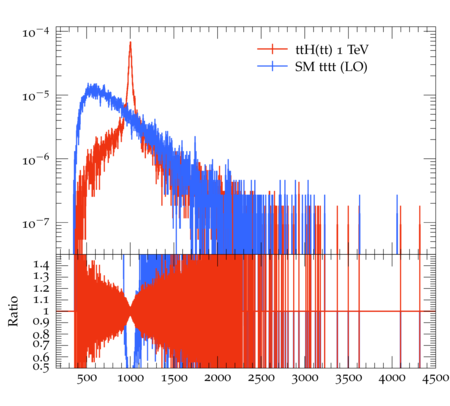
\includegraphics[width=\textwidth]{../plots/ttH_1000/tttt_ttH/Inclusive_InvM_ttbar12.png}\\
\textit{\small Inclusive InvM ttbar12}
\column{0.3\textwidth}
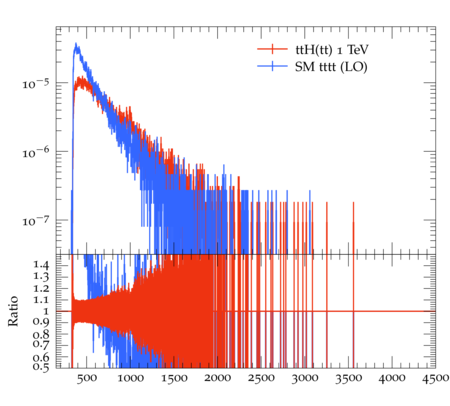
\includegraphics[width=\textwidth]{../plots/ttH_1000/tttt_ttH/Inclusive_InvM_ttbar34.png}\\
\textit{\small Inclusive InvM ttbar34}
\column{0.3\textwidth}
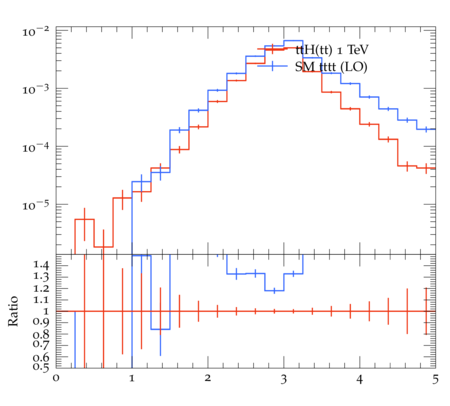
\includegraphics[width=\textwidth]{../plots/ttH_1000/tttt_ttH/Inclusive_dR_ttbar12.png}\\
\textit{\small Inclusive dR ttbar12}
\end{columns}
\end{frame}
\begin{frame}
\frametitle{Sample: ttH 1000 GeV - event level plots}
\begin{columns}
\column{0.3\textwidth}
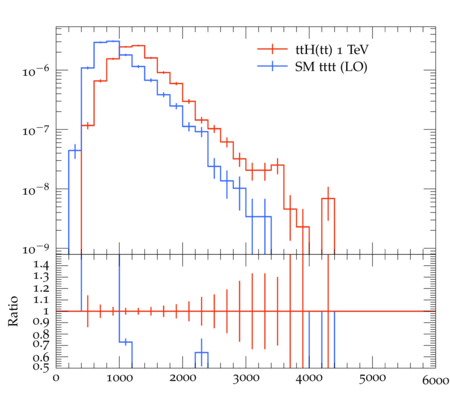
\includegraphics[width=\textwidth]{../plots/ttH_1000/tttt_ttH_1LOS/BaselineSR_HT_3.png}\\
\textit{\small BaselineSR HT 3}
\column{0.3\textwidth}
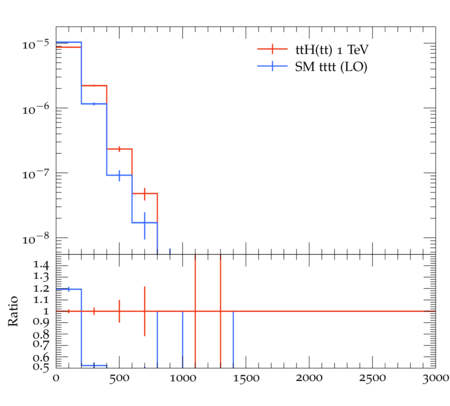
\includegraphics[width=\textwidth]{../plots/ttH_1000/tttt_ttH_1LOS/BaselineSR_MET.png}\\
\textit{\small BaselineSR MET}
\column{0.3\textwidth}
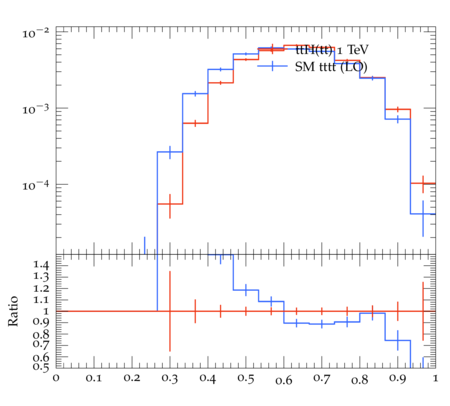
\includegraphics[width=\textwidth]{../plots/ttH_1000/tttt_ttH_1LOS/BaselineSR_centrality.png}\\
\textit{\small BaselineSR centrality}
\end{columns}
\begin{columns}
\column{0.3\textwidth}
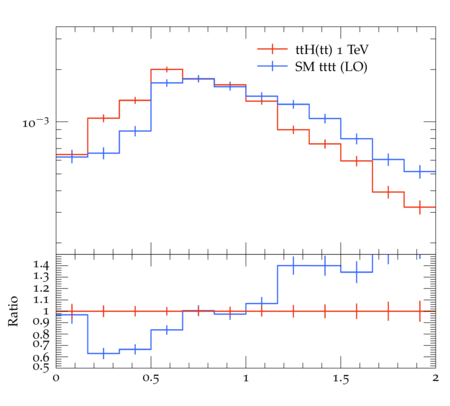
\includegraphics[width=\textwidth]{../plots/ttH_1000/tttt_ttH_1LOS/BaselineSR_deltaR_bl_min.png}\\
\textit{\small BaselineSR deltaR bl min}
\column{0.3\textwidth}
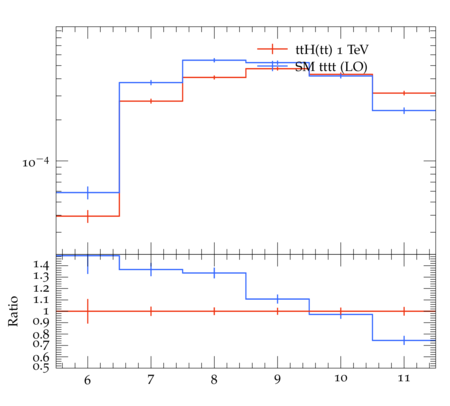
\includegraphics[width=\textwidth]{../plots/ttH_1000/tttt_ttH_1LOS/BaselineSR_nJets.png}\\
\textit{\small BaselineSR nJets}
\column{0.3\textwidth}
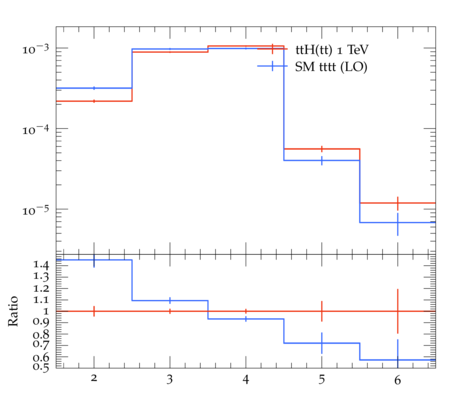
\includegraphics[width=\textwidth]{../plots/ttH_1000/tttt_ttH_1LOS/BaselineSR_nBjets.png}\\
\textit{\small BaselineSR nBjets}
\end{columns}
\end{frame}
\begin{frame}
\frametitle{Sample: ttH 1100 GeV - parton level plots}
\begin{columns}
\column{0.3\textwidth}
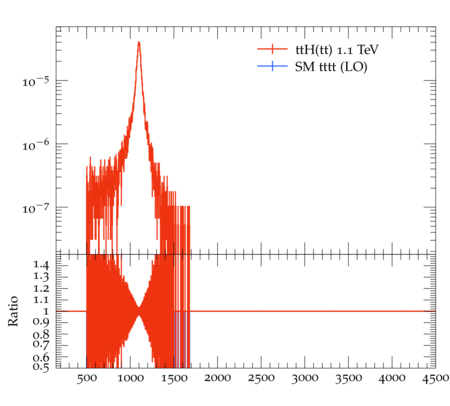
\includegraphics[width=\textwidth]{../plots/ttH_1100/tttt_ttH/Inclusive_mH.png}\\
\textit{\small Inclusive mH}
\column{0.3\textwidth}
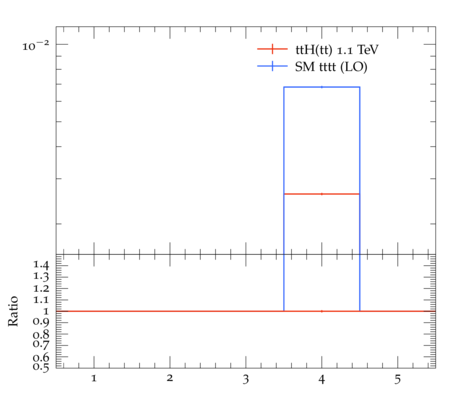
\includegraphics[width=\textwidth]{../plots/ttH_1100/tttt_ttH/Inclusive_nTop.png}\\
\textit{\small Inclusive nTop}
\column{0.3\textwidth}
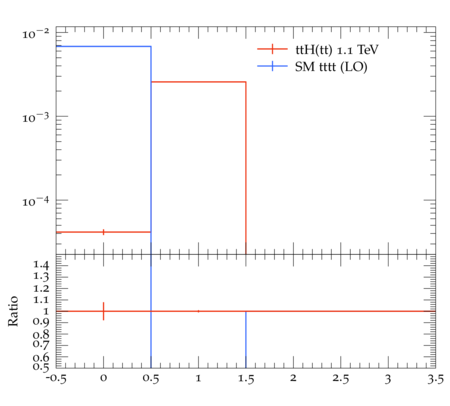
\includegraphics[width=\textwidth]{../plots/ttH_1100/tttt_ttH/Inclusive_nH.png}\\
\textit{\small Inclusive nH}
\end{columns}
\begin{columns}
\column{0.3\textwidth}
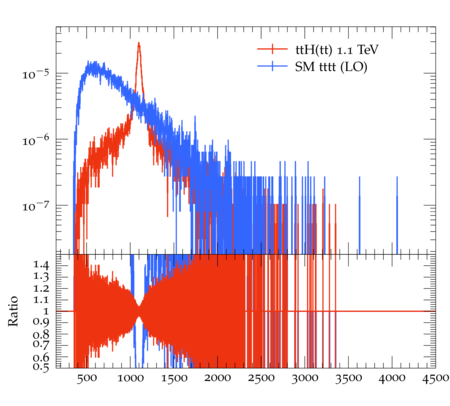
\includegraphics[width=\textwidth]{../plots/ttH_1100/tttt_ttH/Inclusive_InvM_ttbar12.png}\\
\textit{\small Inclusive InvM ttbar12}
\column{0.3\textwidth}
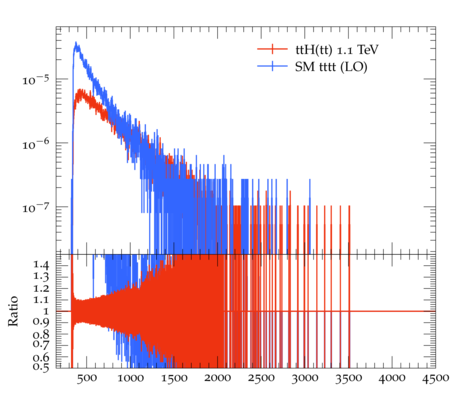
\includegraphics[width=\textwidth]{../plots/ttH_1100/tttt_ttH/Inclusive_InvM_ttbar34.png}\\
\textit{\small Inclusive InvM ttbar34}
\column{0.3\textwidth}
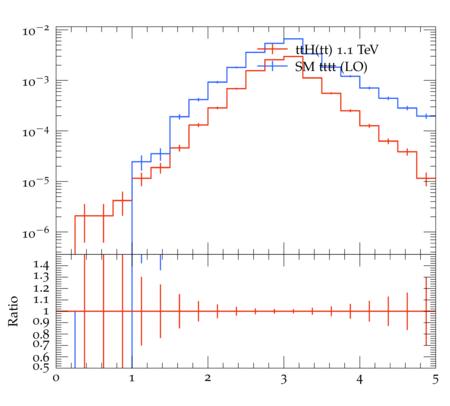
\includegraphics[width=\textwidth]{../plots/ttH_1100/tttt_ttH/Inclusive_dR_ttbar12.png}\\
\textit{\small Inclusive dR ttbar12}
\end{columns}
\end{frame}
\begin{frame}
\frametitle{Sample: ttH 1100 GeV - event level plots}
\begin{columns}
\column{0.3\textwidth}
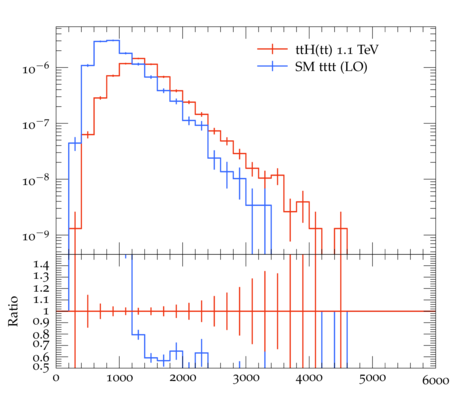
\includegraphics[width=\textwidth]{../plots/ttH_1100/tttt_ttH_1LOS/BaselineSR_HT_3.png}\\
\textit{\small BaselineSR HT 3}
\column{0.3\textwidth}
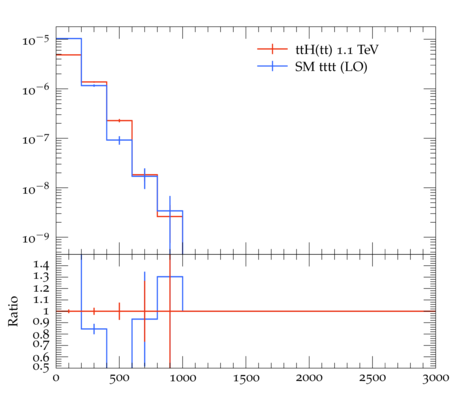
\includegraphics[width=\textwidth]{../plots/ttH_1100/tttt_ttH_1LOS/BaselineSR_MET.png}\\
\textit{\small BaselineSR MET}
\column{0.3\textwidth}
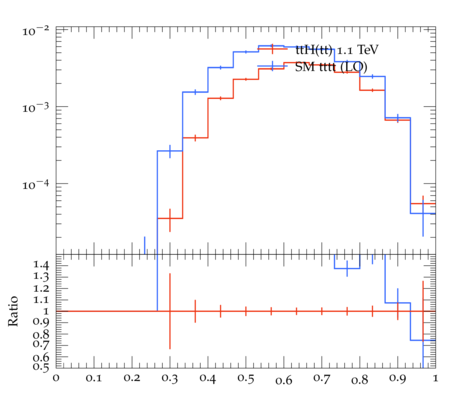
\includegraphics[width=\textwidth]{../plots/ttH_1100/tttt_ttH_1LOS/BaselineSR_centrality.png}\\
\textit{\small BaselineSR centrality}
\end{columns}
\begin{columns}
\column{0.3\textwidth}
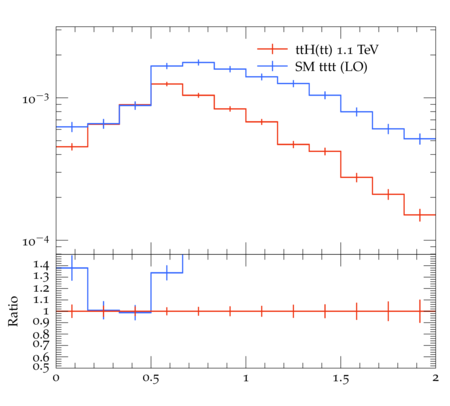
\includegraphics[width=\textwidth]{../plots/ttH_1100/tttt_ttH_1LOS/BaselineSR_deltaR_bl_min.png}\\
\textit{\small BaselineSR deltaR bl min}
\column{0.3\textwidth}
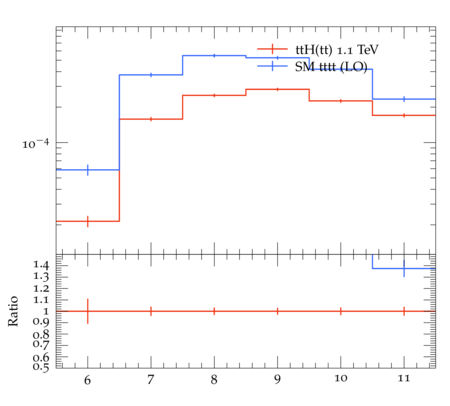
\includegraphics[width=\textwidth]{../plots/ttH_1100/tttt_ttH_1LOS/BaselineSR_nJets.png}\\
\textit{\small BaselineSR nJets}
\column{0.3\textwidth}
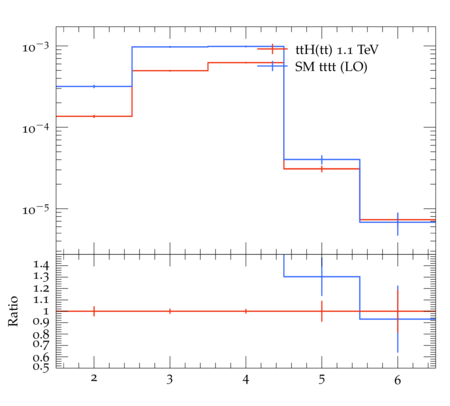
\includegraphics[width=\textwidth]{../plots/ttH_1100/tttt_ttH_1LOS/BaselineSR_nBjets.png}\\
\textit{\small BaselineSR nBjets}
\end{columns}
\end{frame}
\begin{frame}
\frametitle{Sample: ttH 1200 GeV - parton level plots}
\begin{columns}
\column{0.3\textwidth}
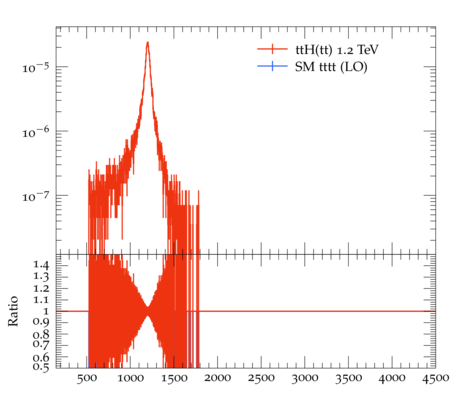
\includegraphics[width=\textwidth]{../plots/ttH_1200/tttt_ttH/Inclusive_mH.png}\\
\textit{\small Inclusive mH}
\column{0.3\textwidth}
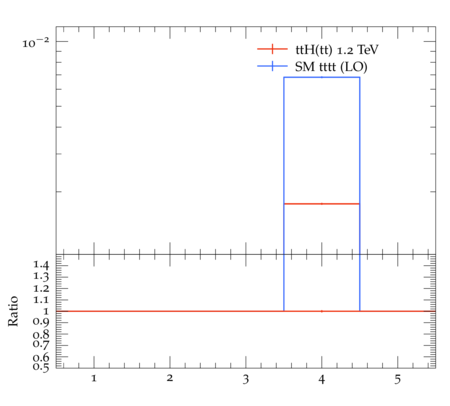
\includegraphics[width=\textwidth]{../plots/ttH_1200/tttt_ttH/Inclusive_nTop.png}\\
\textit{\small Inclusive nTop}
\column{0.3\textwidth}
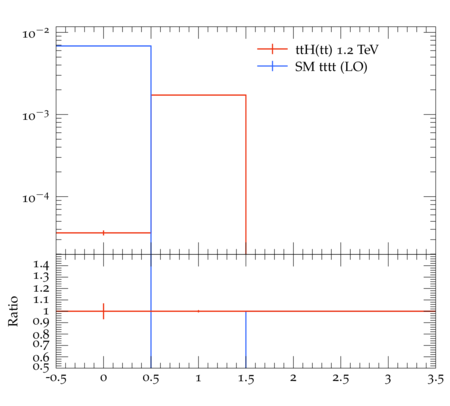
\includegraphics[width=\textwidth]{../plots/ttH_1200/tttt_ttH/Inclusive_nH.png}\\
\textit{\small Inclusive nH}
\end{columns}
\begin{columns}
\column{0.3\textwidth}
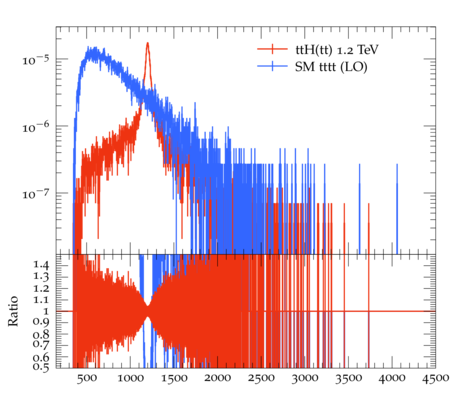
\includegraphics[width=\textwidth]{../plots/ttH_1200/tttt_ttH/Inclusive_InvM_ttbar12.png}\\
\textit{\small Inclusive InvM ttbar12}
\column{0.3\textwidth}
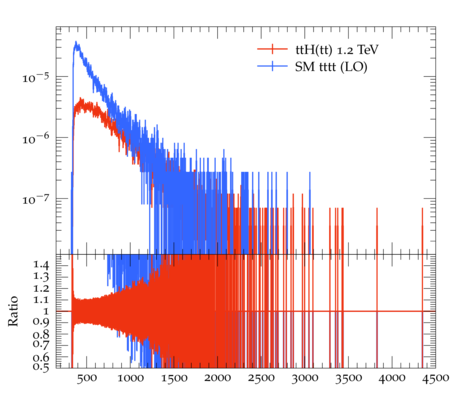
\includegraphics[width=\textwidth]{../plots/ttH_1200/tttt_ttH/Inclusive_InvM_ttbar34.png}\\
\textit{\small Inclusive InvM ttbar34}
\column{0.3\textwidth}
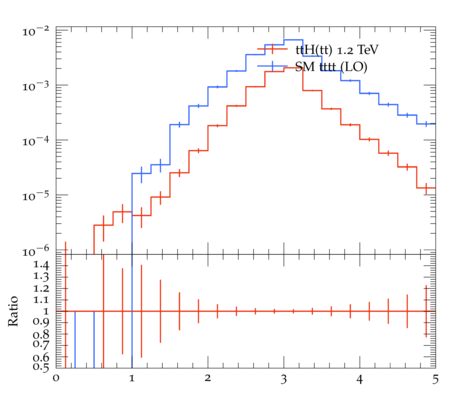
\includegraphics[width=\textwidth]{../plots/ttH_1200/tttt_ttH/Inclusive_dR_ttbar12.png}\\
\textit{\small Inclusive dR ttbar12}
\end{columns}
\end{frame}
\begin{frame}
\frametitle{Sample: ttH 1200 GeV - event level plots}
\begin{columns}
\column{0.3\textwidth}
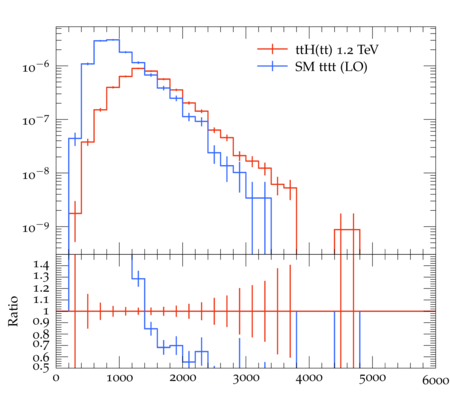
\includegraphics[width=\textwidth]{../plots/ttH_1200/tttt_ttH_1LOS/BaselineSR_HT_3.png}\\
\textit{\small BaselineSR HT 3}
\column{0.3\textwidth}
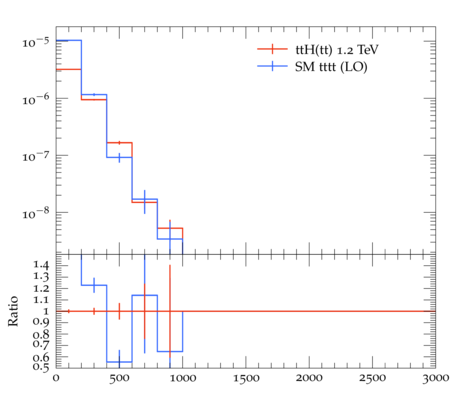
\includegraphics[width=\textwidth]{../plots/ttH_1200/tttt_ttH_1LOS/BaselineSR_MET.png}\\
\textit{\small BaselineSR MET}
\column{0.3\textwidth}
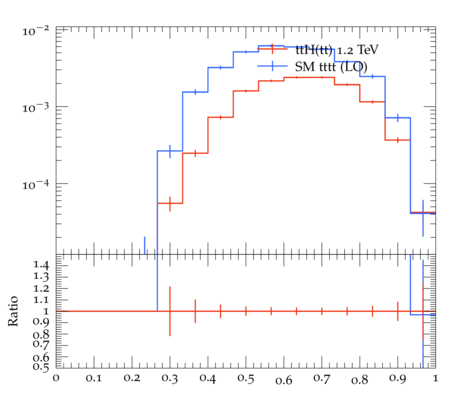
\includegraphics[width=\textwidth]{../plots/ttH_1200/tttt_ttH_1LOS/BaselineSR_centrality.png}\\
\textit{\small BaselineSR centrality}
\end{columns}
\begin{columns}
\column{0.3\textwidth}
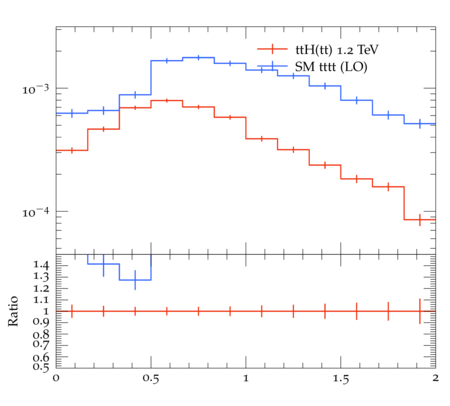
\includegraphics[width=\textwidth]{../plots/ttH_1200/tttt_ttH_1LOS/BaselineSR_deltaR_bl_min.png}\\
\textit{\small BaselineSR deltaR bl min}
\column{0.3\textwidth}
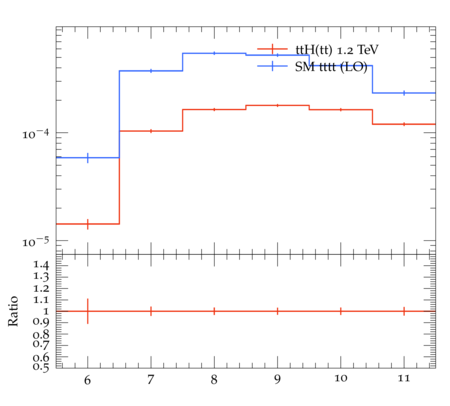
\includegraphics[width=\textwidth]{../plots/ttH_1200/tttt_ttH_1LOS/BaselineSR_nJets.png}\\
\textit{\small BaselineSR nJets}
\column{0.3\textwidth}
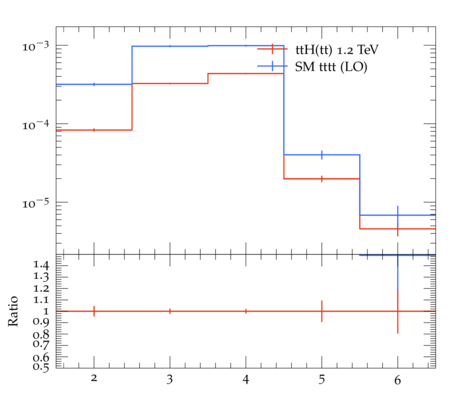
\includegraphics[width=\textwidth]{../plots/ttH_1200/tttt_ttH_1LOS/BaselineSR_nBjets.png}\\
\textit{\small BaselineSR nBjets}
\end{columns}
\end{frame}
\begin{frame}
\frametitle{Sample: ttH 1300 GeV - parton level plots}
\begin{columns}
\column{0.3\textwidth}
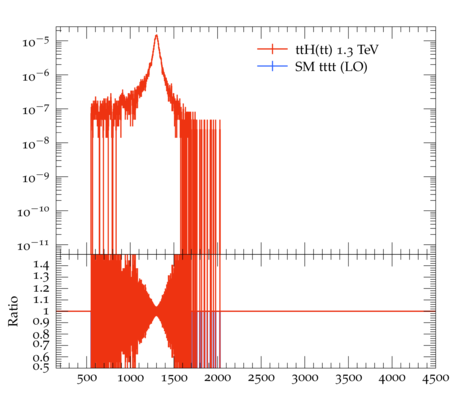
\includegraphics[width=\textwidth]{../plots/ttH_1300/tttt_ttH/Inclusive_mH.png}\\
\textit{\small Inclusive mH}
\column{0.3\textwidth}
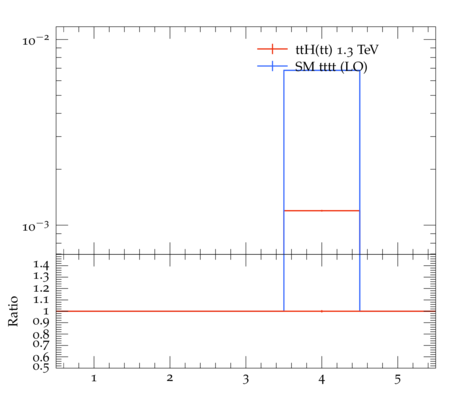
\includegraphics[width=\textwidth]{../plots/ttH_1300/tttt_ttH/Inclusive_nTop.png}\\
\textit{\small Inclusive nTop}
\column{0.3\textwidth}
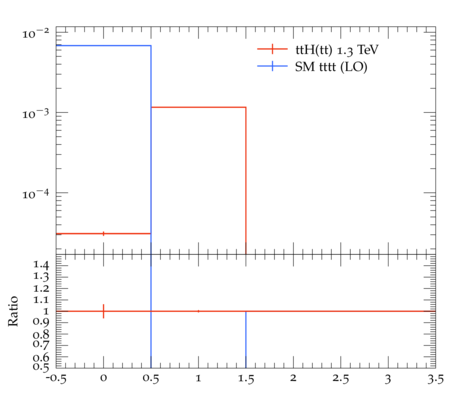
\includegraphics[width=\textwidth]{../plots/ttH_1300/tttt_ttH/Inclusive_nH.png}\\
\textit{\small Inclusive nH}
\end{columns}
\begin{columns}
\column{0.3\textwidth}
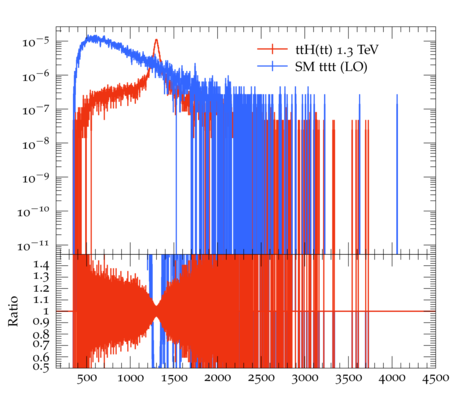
\includegraphics[width=\textwidth]{../plots/ttH_1300/tttt_ttH/Inclusive_InvM_ttbar12.png}\\
\textit{\small Inclusive InvM ttbar12}
\column{0.3\textwidth}
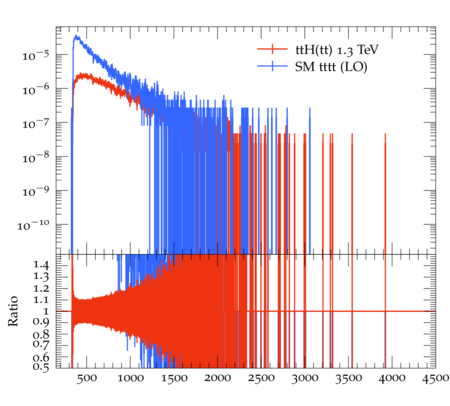
\includegraphics[width=\textwidth]{../plots/ttH_1300/tttt_ttH/Inclusive_InvM_ttbar34.png}\\
\textit{\small Inclusive InvM ttbar34}
\column{0.3\textwidth}
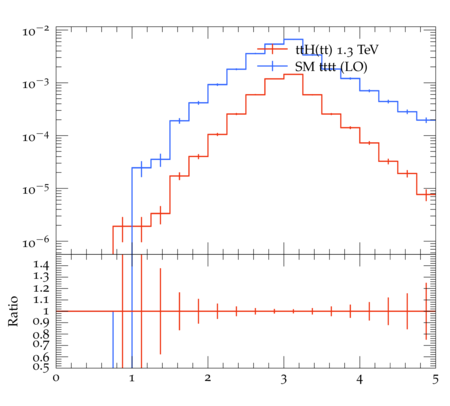
\includegraphics[width=\textwidth]{../plots/ttH_1300/tttt_ttH/Inclusive_dR_ttbar12.png}\\
\textit{\small Inclusive dR ttbar12}
\end{columns}
\end{frame}
\begin{frame}
\frametitle{Sample: ttH 1300 GeV - event level plots}
\begin{columns}
\column{0.3\textwidth}
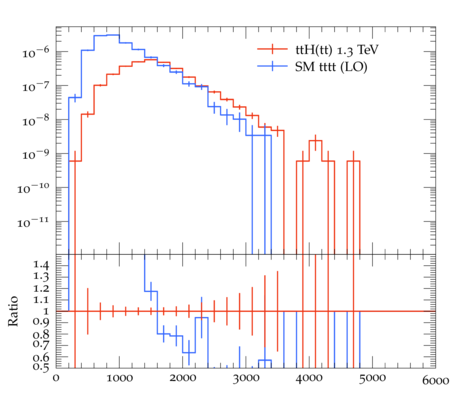
\includegraphics[width=\textwidth]{../plots/ttH_1300/tttt_ttH_1LOS/BaselineSR_HT_3.png}\\
\textit{\small BaselineSR HT 3}
\column{0.3\textwidth}
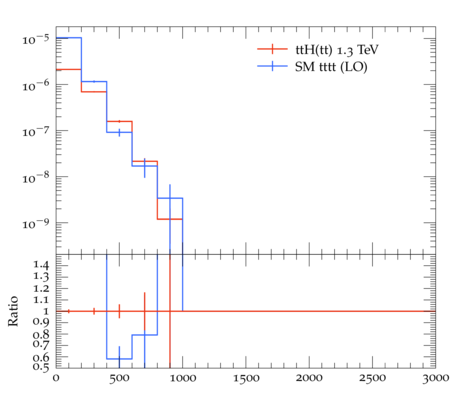
\includegraphics[width=\textwidth]{../plots/ttH_1300/tttt_ttH_1LOS/BaselineSR_MET.png}\\
\textit{\small BaselineSR MET}
\column{0.3\textwidth}
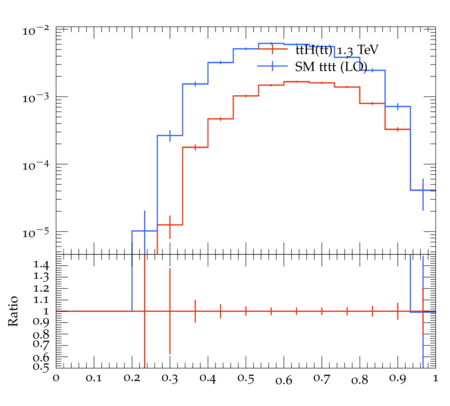
\includegraphics[width=\textwidth]{../plots/ttH_1300/tttt_ttH_1LOS/BaselineSR_centrality.png}\\
\textit{\small BaselineSR centrality}
\end{columns}
\begin{columns}
\column{0.3\textwidth}
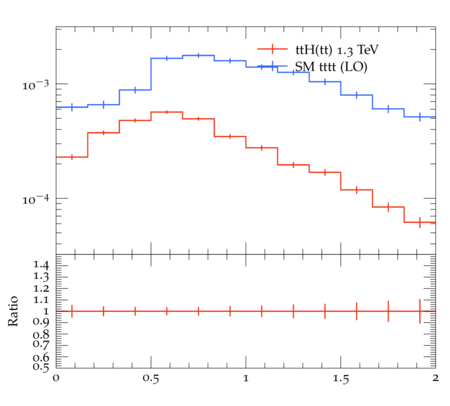
\includegraphics[width=\textwidth]{../plots/ttH_1300/tttt_ttH_1LOS/BaselineSR_deltaR_bl_min.png}\\
\textit{\small BaselineSR deltaR bl min}
\column{0.3\textwidth}
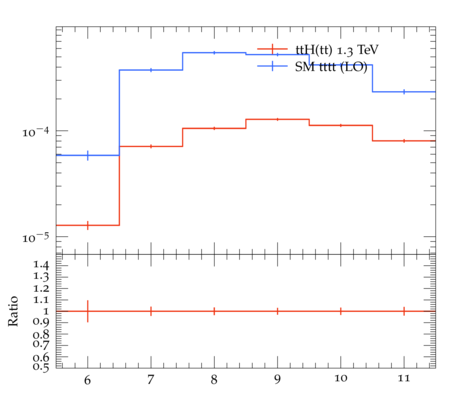
\includegraphics[width=\textwidth]{../plots/ttH_1300/tttt_ttH_1LOS/BaselineSR_nJets.png}\\
\textit{\small BaselineSR nJets}
\column{0.3\textwidth}
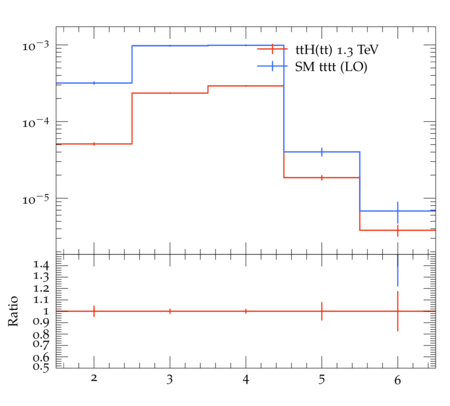
\includegraphics[width=\textwidth]{../plots/ttH_1300/tttt_ttH_1LOS/BaselineSR_nBjets.png}\\
\textit{\small BaselineSR nBjets}
\end{columns}
\end{frame}
\begin{frame}
\frametitle{Sample: ttH 1400 GeV - parton level plots}
\begin{columns}
\column{0.3\textwidth}
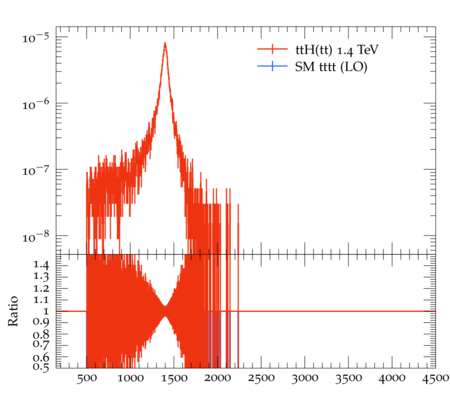
\includegraphics[width=\textwidth]{../plots/ttH_1400/tttt_ttH/Inclusive_mH.png}\\
\textit{\small Inclusive mH}
\column{0.3\textwidth}
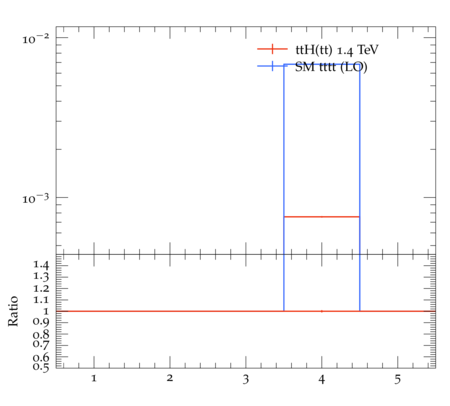
\includegraphics[width=\textwidth]{../plots/ttH_1400/tttt_ttH/Inclusive_nTop.png}\\
\textit{\small Inclusive nTop}
\column{0.3\textwidth}
\includegraphics[width=\textwidth]{../plots/ttH_1400/tttt_ttH/Inclusive_nH.png}\\
\textit{\small Inclusive nH}
\end{columns}
\begin{columns}
\column{0.3\textwidth}
\includegraphics[width=\textwidth]{../plots/ttH_1400/tttt_ttH/Inclusive_InvM_ttbar12.png}\\
\textit{\small Inclusive InvM ttbar12}
\column{0.3\textwidth}
\includegraphics[width=\textwidth]{../plots/ttH_1400/tttt_ttH/Inclusive_InvM_ttbar34.png}\\
\textit{\small Inclusive InvM ttbar34}
\column{0.3\textwidth}
\includegraphics[width=\textwidth]{../plots/ttH_1400/tttt_ttH/Inclusive_dR_ttbar12.png}\\
\textit{\small Inclusive dR ttbar12}
\end{columns}
\end{frame}
\begin{frame}
\frametitle{Sample: ttH 1400 GeV - event level plots}
\begin{columns}
\column{0.3\textwidth}
\includegraphics[width=\textwidth]{../plots/ttH_1400/tttt_ttH_1LOS/BaselineSR_HT_3.png}\\
\textit{\small BaselineSR HT 3}
\column{0.3\textwidth}
\includegraphics[width=\textwidth]{../plots/ttH_1400/tttt_ttH_1LOS/BaselineSR_MET.png}\\
\textit{\small BaselineSR MET}
\column{0.3\textwidth}
\includegraphics[width=\textwidth]{../plots/ttH_1400/tttt_ttH_1LOS/BaselineSR_centrality.png}\\
\textit{\small BaselineSR centrality}
\end{columns}
\begin{columns}
\column{0.3\textwidth}
\includegraphics[width=\textwidth]{../plots/ttH_1400/tttt_ttH_1LOS/BaselineSR_deltaR_bl_min.png}\\
\textit{\small BaselineSR deltaR bl min}
\column{0.3\textwidth}
\includegraphics[width=\textwidth]{../plots/ttH_1400/tttt_ttH_1LOS/BaselineSR_nJets.png}\\
\textit{\small BaselineSR nJets}
\column{0.3\textwidth}
\includegraphics[width=\textwidth]{../plots/ttH_1400/tttt_ttH_1LOS/BaselineSR_nBjets.png}\\
\textit{\small BaselineSR nBjets}
\end{columns}
\end{frame}
\begin{frame}
\frametitle{Sample: ttH 1500 GeV - parton level plots}
\begin{columns}
\column{0.3\textwidth}
\includegraphics[width=\textwidth]{../plots/ttH_1500/tttt_ttH/Inclusive_mH.png}\\
\textit{\small Inclusive mH}
\column{0.3\textwidth}
\includegraphics[width=\textwidth]{../plots/ttH_1500/tttt_ttH/Inclusive_nTop.png}\\
\textit{\small Inclusive nTop}
\column{0.3\textwidth}
\includegraphics[width=\textwidth]{../plots/ttH_1500/tttt_ttH/Inclusive_nH.png}\\
\textit{\small Inclusive nH}
\end{columns}
\begin{columns}
\column{0.3\textwidth}
\includegraphics[width=\textwidth]{../plots/ttH_1500/tttt_ttH/Inclusive_InvM_ttbar12.png}\\
\textit{\small Inclusive InvM ttbar12}
\column{0.3\textwidth}
\includegraphics[width=\textwidth]{../plots/ttH_1500/tttt_ttH/Inclusive_InvM_ttbar34.png}\\
\textit{\small Inclusive InvM ttbar34}
\column{0.3\textwidth}
\includegraphics[width=\textwidth]{../plots/ttH_1500/tttt_ttH/Inclusive_dR_ttbar12.png}\\
\textit{\small Inclusive dR ttbar12}
\end{columns}
\end{frame}
\begin{frame}
\frametitle{Sample: ttH 1500 GeV - event level plots}
\begin{columns}
\column{0.3\textwidth}
\includegraphics[width=\textwidth]{../plots/ttH_1500/tttt_ttH_1LOS/BaselineSR_HT_3.png}\\
\textit{\small BaselineSR HT 3}
\column{0.3\textwidth}
\includegraphics[width=\textwidth]{../plots/ttH_1500/tttt_ttH_1LOS/BaselineSR_MET.png}\\
\textit{\small BaselineSR MET}
\column{0.3\textwidth}
\includegraphics[width=\textwidth]{../plots/ttH_1500/tttt_ttH_1LOS/BaselineSR_centrality.png}\\
\textit{\small BaselineSR centrality}
\end{columns}
\begin{columns}
\column{0.3\textwidth}
\includegraphics[width=\textwidth]{../plots/ttH_1500/tttt_ttH_1LOS/BaselineSR_deltaR_bl_min.png}\\
\textit{\small BaselineSR deltaR bl min}
\column{0.3\textwidth}
\includegraphics[width=\textwidth]{../plots/ttH_1500/tttt_ttH_1LOS/BaselineSR_nJets.png}\\
\textit{\small BaselineSR nJets}
\column{0.3\textwidth}
\includegraphics[width=\textwidth]{../plots/ttH_1500/tttt_ttH_1LOS/BaselineSR_nBjets.png}\\
\textit{\small BaselineSR nBjets}
\end{columns}
\end{frame}
\begin{frame}
\frametitle{Sample: ttH 1750 GeV - parton level plots}
\begin{columns}
\column{0.3\textwidth}
\includegraphics[width=\textwidth]{../plots/ttH_1750/tttt_ttH/Inclusive_mH.png}\\
\textit{\small Inclusive mH}
\column{0.3\textwidth}
\includegraphics[width=\textwidth]{../plots/ttH_1750/tttt_ttH/Inclusive_nTop.png}\\
\textit{\small Inclusive nTop}
\column{0.3\textwidth}
\includegraphics[width=\textwidth]{../plots/ttH_1750/tttt_ttH/Inclusive_nH.png}\\
\textit{\small Inclusive nH}
\end{columns}
\begin{columns}
\column{0.3\textwidth}
\includegraphics[width=\textwidth]{../plots/ttH_1750/tttt_ttH/Inclusive_InvM_ttbar12.png}\\
\textit{\small Inclusive InvM ttbar12}
\column{0.3\textwidth}
\includegraphics[width=\textwidth]{../plots/ttH_1750/tttt_ttH/Inclusive_InvM_ttbar34.png}\\
\textit{\small Inclusive InvM ttbar34}
\column{0.3\textwidth}
\includegraphics[width=\textwidth]{../plots/ttH_1750/tttt_ttH/Inclusive_dR_ttbar12.png}\\
\textit{\small Inclusive dR ttbar12}
\end{columns}
\end{frame}
\begin{frame}
\frametitle{Sample: ttH 1750 GeV - event level plots}
\begin{columns}
\column{0.3\textwidth}
\includegraphics[width=\textwidth]{../plots/ttH_1750/tttt_ttH_1LOS/BaselineSR_HT_3.png}\\
\textit{\small BaselineSR HT 3}
\column{0.3\textwidth}
\includegraphics[width=\textwidth]{../plots/ttH_1750/tttt_ttH_1LOS/BaselineSR_MET.png}\\
\textit{\small BaselineSR MET}
\column{0.3\textwidth}
\includegraphics[width=\textwidth]{../plots/ttH_1750/tttt_ttH_1LOS/BaselineSR_centrality.png}\\
\textit{\small BaselineSR centrality}
\end{columns}
\begin{columns}
\column{0.3\textwidth}
\includegraphics[width=\textwidth]{../plots/ttH_1750/tttt_ttH_1LOS/BaselineSR_deltaR_bl_min.png}\\
\textit{\small BaselineSR deltaR bl min}
\column{0.3\textwidth}
\includegraphics[width=\textwidth]{../plots/ttH_1750/tttt_ttH_1LOS/BaselineSR_nJets.png}\\
\textit{\small BaselineSR nJets}
\column{0.3\textwidth}
\includegraphics[width=\textwidth]{../plots/ttH_1750/tttt_ttH_1LOS/BaselineSR_nBjets.png}\\
\textit{\small BaselineSR nBjets}
\end{columns}
\end{frame}
\begin{frame}
\frametitle{Sample: ttH 2000 GeV - parton level plots}
\begin{columns}
\column{0.3\textwidth}
\includegraphics[width=\textwidth]{../plots/ttH_2000/tttt_ttH/Inclusive_mH.png}\\
\textit{\small Inclusive mH}
\column{0.3\textwidth}
\includegraphics[width=\textwidth]{../plots/ttH_2000/tttt_ttH/Inclusive_nTop.png}\\
\textit{\small Inclusive nTop}
\column{0.3\textwidth}
\includegraphics[width=\textwidth]{../plots/ttH_2000/tttt_ttH/Inclusive_nH.png}\\
\textit{\small Inclusive nH}
\end{columns}
\begin{columns}
\column{0.3\textwidth}
\includegraphics[width=\textwidth]{../plots/ttH_2000/tttt_ttH/Inclusive_InvM_ttbar12.png}\\
\textit{\small Inclusive InvM ttbar12}
\column{0.3\textwidth}
\includegraphics[width=\textwidth]{../plots/ttH_2000/tttt_ttH/Inclusive_InvM_ttbar34.png}\\
\textit{\small Inclusive InvM ttbar34}
\column{0.3\textwidth}
\includegraphics[width=\textwidth]{../plots/ttH_2000/tttt_ttH/Inclusive_dR_ttbar12.png}\\
\textit{\small Inclusive dR ttbar12}
\end{columns}
\end{frame}
\begin{frame}
\frametitle{Sample: ttH 2000 GeV - event level plots}
\begin{columns}
\column{0.3\textwidth}
\includegraphics[width=\textwidth]{../plots/ttH_2000/tttt_ttH_1LOS/BaselineSR_HT_3.png}\\
\textit{\small BaselineSR HT 3}
\column{0.3\textwidth}
\includegraphics[width=\textwidth]{../plots/ttH_2000/tttt_ttH_1LOS/BaselineSR_MET.png}\\
\textit{\small BaselineSR MET}
\column{0.3\textwidth}
\includegraphics[width=\textwidth]{../plots/ttH_2000/tttt_ttH_1LOS/BaselineSR_centrality.png}\\
\textit{\small BaselineSR centrality}
\end{columns}
\begin{columns}
\column{0.3\textwidth}
\includegraphics[width=\textwidth]{../plots/ttH_2000/tttt_ttH_1LOS/BaselineSR_deltaR_bl_min.png}\\
\textit{\small BaselineSR deltaR bl min}
\column{0.3\textwidth}
\includegraphics[width=\textwidth]{../plots/ttH_2000/tttt_ttH_1LOS/BaselineSR_nJets.png}\\
\textit{\small BaselineSR nJets}
\column{0.3\textwidth}
\includegraphics[width=\textwidth]{../plots/ttH_2000/tttt_ttH_1LOS/BaselineSR_nBjets.png}\\
\textit{\small BaselineSR nBjets}
\end{columns}
\end{frame}
\begin{frame}
\frametitle{Sample: ttH 2250 GeV - parton level plots}
\begin{columns}
\column{0.3\textwidth}
\includegraphics[width=\textwidth]{../plots/ttH_2250/tttt_ttH/Inclusive_mH.png}\\
\textit{\small Inclusive mH}
\column{0.3\textwidth}
\includegraphics[width=\textwidth]{../plots/ttH_2250/tttt_ttH/Inclusive_nTop.png}\\
\textit{\small Inclusive nTop}
\column{0.3\textwidth}
\includegraphics[width=\textwidth]{../plots/ttH_2250/tttt_ttH/Inclusive_nH.png}\\
\textit{\small Inclusive nH}
\end{columns}
\begin{columns}
\column{0.3\textwidth}
\includegraphics[width=\textwidth]{../plots/ttH_2250/tttt_ttH/Inclusive_InvM_ttbar12.png}\\
\textit{\small Inclusive InvM ttbar12}
\column{0.3\textwidth}
\includegraphics[width=\textwidth]{../plots/ttH_2250/tttt_ttH/Inclusive_InvM_ttbar34.png}\\
\textit{\small Inclusive InvM ttbar34}
\column{0.3\textwidth}
\includegraphics[width=\textwidth]{../plots/ttH_2250/tttt_ttH/Inclusive_dR_ttbar12.png}\\
\textit{\small Inclusive dR ttbar12}
\end{columns}
\end{frame}
\begin{frame}
\frametitle{Sample: ttH 2250 GeV - event level plots}
\begin{columns}
\column{0.3\textwidth}
\includegraphics[width=\textwidth]{../plots/ttH_2250/tttt_ttH_1LOS/BaselineSR_HT_3.png}\\
\textit{\small BaselineSR HT 3}
\column{0.3\textwidth}
\includegraphics[width=\textwidth]{../plots/ttH_2250/tttt_ttH_1LOS/BaselineSR_MET.png}\\
\textit{\small BaselineSR MET}
\column{0.3\textwidth}
\includegraphics[width=\textwidth]{../plots/ttH_2250/tttt_ttH_1LOS/BaselineSR_centrality.png}\\
\textit{\small BaselineSR centrality}
\end{columns}
\begin{columns}
\column{0.3\textwidth}
\includegraphics[width=\textwidth]{../plots/ttH_2250/tttt_ttH_1LOS/BaselineSR_deltaR_bl_min.png}\\
\textit{\small BaselineSR deltaR bl min}
\column{0.3\textwidth}
\includegraphics[width=\textwidth]{../plots/ttH_2250/tttt_ttH_1LOS/BaselineSR_nJets.png}\\
\textit{\small BaselineSR nJets}
\column{0.3\textwidth}
\includegraphics[width=\textwidth]{../plots/ttH_2250/tttt_ttH_1LOS/BaselineSR_nBjets.png}\\
\textit{\small BaselineSR nBjets}
\end{columns}
\end{frame}
\begin{frame}
\frametitle{Sample: ttH 2500 GeV - parton level plots}
\begin{columns}
\column{0.3\textwidth}
\includegraphics[width=\textwidth]{../plots/ttH_2500/tttt_ttH/Inclusive_mH.png}\\
\textit{\small Inclusive mH}
\column{0.3\textwidth}
\includegraphics[width=\textwidth]{../plots/ttH_2500/tttt_ttH/Inclusive_nTop.png}\\
\textit{\small Inclusive nTop}
\column{0.3\textwidth}
\includegraphics[width=\textwidth]{../plots/ttH_2500/tttt_ttH/Inclusive_nH.png}\\
\textit{\small Inclusive nH}
\end{columns}
\begin{columns}
\column{0.3\textwidth}
\includegraphics[width=\textwidth]{../plots/ttH_2500/tttt_ttH/Inclusive_InvM_ttbar12.png}\\
\textit{\small Inclusive InvM ttbar12}
\column{0.3\textwidth}
\includegraphics[width=\textwidth]{../plots/ttH_2500/tttt_ttH/Inclusive_InvM_ttbar34.png}\\
\textit{\small Inclusive InvM ttbar34}
\column{0.3\textwidth}
\includegraphics[width=\textwidth]{../plots/ttH_2500/tttt_ttH/Inclusive_dR_ttbar12.png}\\
\textit{\small Inclusive dR ttbar12}
\end{columns}
\end{frame}
\begin{frame}
\frametitle{Sample: ttH 2500 GeV - event level plots}
\begin{columns}
\column{0.3\textwidth}
\includegraphics[width=\textwidth]{../plots/ttH_2500/tttt_ttH_1LOS/BaselineSR_HT_3.png}\\
\textit{\small BaselineSR HT 3}
\column{0.3\textwidth}
\includegraphics[width=\textwidth]{../plots/ttH_2500/tttt_ttH_1LOS/BaselineSR_MET.png}\\
\textit{\small BaselineSR MET}
\column{0.3\textwidth}
\includegraphics[width=\textwidth]{../plots/ttH_2500/tttt_ttH_1LOS/BaselineSR_centrality.png}\\
\textit{\small BaselineSR centrality}
\end{columns}
\begin{columns}
\column{0.3\textwidth}
\includegraphics[width=\textwidth]{../plots/ttH_2500/tttt_ttH_1LOS/BaselineSR_deltaR_bl_min.png}\\
\textit{\small BaselineSR deltaR bl min}
\column{0.3\textwidth}
\includegraphics[width=\textwidth]{../plots/ttH_2500/tttt_ttH_1LOS/BaselineSR_nJets.png}\\
\textit{\small BaselineSR nJets}
\column{0.3\textwidth}
\includegraphics[width=\textwidth]{../plots/ttH_2500/tttt_ttH_1LOS/BaselineSR_nBjets.png}\\
\textit{\small BaselineSR nBjets}
\end{columns}
\end{frame}
\end{document}
